\chapter{Work Done}

\section{Progress Made By Project Final}

\subsection{Image Slicing}
The data drawn from the Kinect is in 2D depth image format. Which is a grey-scale image where the distances of all points are represented by a single value. The closer the surface the brighter it shows on the image.

The problem with the structure of the raw data is, when the objects are very close or very similar in height the differences corresponding to respective surfaces become too subtle to extract object from. In those cases the data raises false positives.

To alleviate this, we used image slicing. Image slicing is an image processing technique where pixel values outside certain regions are reduced to zero.

As shown in figure \ref{fig:label31}, by fading all areas outside a certain region to black objects within that region are depicted with much more contrast since the dynamic range is focussed on a much smaller area. 

With this false negative are removed but the calibration is of utmost importance. If the regions near and far borders are not determined properly desired objects are lost completely.
\subsection{Blob Tracking}
As the main aim of the project is object tracking, we directed most of our effort to this area.

Once the depth image from the Kinect is cleaned up we extract the contours of the image and encapsulate them in rectangles which are inner representations of the captured objects as shown in figure \ref{fig:label31}. Keeping track of more than one blobs and matching rats with their respective blob is made with the help of cages which are shown as green rectangles.

This part is implemented with the help of OpenCv libraries which provides helper functions for both jobs: extracting contours and marking them.
\begin{figure}[htb]
\centering
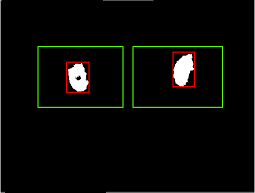
\includegraphics[scale=2]{./track} % e.g. insert ./image for image.png in the working directory, adjust scale as necessary
\caption{Sliced image with rats marked red and cages marked green}
\label{fig:label31} % insert suitable label, this is used to refer to a fig from within the text as shown above
\end{figure}
\subsection{User Interface}
User interface is built to prepare experiments, record videos and track objects with Kinect. This program while recording the processed video and gathering data, slices the image, isolates the objects. 
\begin{figure}[htb]
\centering
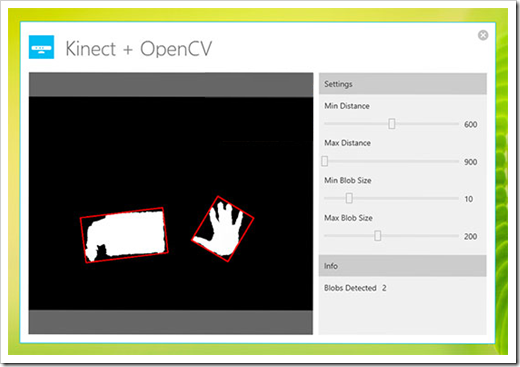
\includegraphics[scale=1]{./UI} % e.g. insert ./image for image.png in the working directory, adjust scale as necessary
\caption{User Interface}
\label{fig:label32} % insert suitable label, this is used to refer to a fig from within the text as shown above
\end{figure}

As shown in figure \ref{fig:label32}, the relevant UI element are the sliders to calibrate far and near borders for the slicer and max/min blob sizes. As of now, calibration of these variables are done by hand and are very important to properly isolate objects to be tracked. Currently, the Psychobiology lab has yet to give us the go ahead for the deployment of our system, so the UI has those sliders left for the calibration purposes. This unfortunately clutters the UI but will be remedied once calibrations and on-site long-term testing is done.

We have also added experiment creation utilities for the use of researchers. This is kept as simple as possible to encourage usage. By using these utilities, the user can choose up to 4 cages and mark them, specify the frequency of data gathering, and other specifications about the experiment. At the end of this creation process, the program also outputs a config file to accompany the experiment. This config file contains all specifications user made and it is helpful for not repeating the same procedures when the experiment is repeated.

By using the buttons of Start, the user can start and stop the experiment at will. Recording is left as an option as well because for some researchers, movement data will be enough for the experiment and video recording will not be needed.
\subsection{Position Data Gathering}
As the project is for experimentation, we needed to get some real world coordinate definition to determine and record movements of rats. For this reason, we have used the built-in skeleton tracking module of Kinect which works in real world coordinates to determine the height of humans. Our program uses this module to compute the movement vectors of rat in meters and record the distance.

The results are recorded in .csv files for extensive usage because Excel has some limitations for number of data points recorded. The position data gathered is presented to the user in raw form and also in a candle-wick graph describing the speed at which a subject moves within a given period as a indicator of a subject’s level of activity.

This software will provide users with all data such as: 
\begin{itemize}
\item mean of position
\item standard deviation of position
\item position history
\item active time periods
\item inactive time periods
\item areas highly frequented by the subject animal
\end{itemize}
and any other report our product owners may require.

\subsection{Multi-Threading}
For performance purposes we chose to separate video record and object tracking functionality to their own threads. This significantly improved performance as these functions were no longer impeded by each other and the UI load.

